In questa sezione viene presentato il prospetto economico in cui vengono riportate le spese effettivamente sostenute. Si riportano le ore impiegate per svolgere le attività programmate, sia per ruolo che per membro del gruppo. In base alla differenza ottenuta tra preventivo e consuntivo, detta conguaglio, si avrà un bilancio:
\begin{itemize}
	\item \textbf{Positivo:} se il preventivo ha superato il consuntivo; 
	\item \textbf{Negativo:} se il consuntivo ha superato il preventivo;
	\item \textbf{In pari:} se consuntivo e preventivo coincidono.
\end{itemize}

\subsection{Analisi}
Si riporta di seguito il consuntivo del periodo di \textit{Analisi}.

\noindent La seguente tabella riporta la differenza di ore impiegate rispetto a quanto preventivato, divise per ruolo. I valori negativi nella tabella indicano un monte ore maggiore di quello preventivato, i valori positivi una diminuzione di ore.

\begin{table}[h]
\centering
\begin{tabular}{|l|c|c|}
	\toprule
	\textbf{Ruolo} & \textbf{Ore per ruolo} & \textbf{Costo per ruolo} \\
	
	\midrule
	Responsabile di Progetto & 1 & 30 \\
	Amministratore di Progetto & 1 & 20 \\ 
	Analista & -2 & -50 \\
	Progettista & & \\
	Programmatore & & \\
	Verificatore & -1 & -15 \\
	\midrule
	\textbf{Totale} & -1 & -15 \\
		
	\bottomrule
\end{tabular}
\caption{Differenza ore e costo per ruolo, Analisi}
\label{tab3}
\end{table} 

\noindent La seguente tabella riporta le differenze tra ore preventivate e quelle impiegate, per membro, durante il periodo di \textit{Analisi}: 
\begin{table}[h]
\centering
\begin{tabular}{|l|c|c|c|c|c|c|c|}
	\toprule
	\textbf{Cognome e Nome} & \multicolumn{6}{c}{\textbf{Ore per ruolo}} & \textbf{Ore Totali} \\
	& \textbf{Re} & \textbf{Am} & \textbf{An} & \textbf{Pt} & \textbf{Pr} & \textbf{Ve} & \\
		
	\midrule
	Agostinetto Matteo & & & -1 & & & & -1 \\
	Burlin Valerio & 1 & & & & & & 1 \\ 
	Carraro Nicola & & & -1 & & & & -1 \\
	Crespan Emanuele & & 1 & & & & & 1 \\
	Ros Fabio & & & & & & & \\
	Suierica Bogdan & & & & & & -1 & -1 \\
		
	\bottomrule
\end{tabular}
\caption{Differenza ore a componente per ruolo, Analisi}
\end{table}

\newpage
\noindent Il seguente grafico riporta la differenza tra le ore preventivate e quelle impiegate, per ruolo, durante il periodo di \textit{Analisi}:
\begin{figure}[h]
\centering
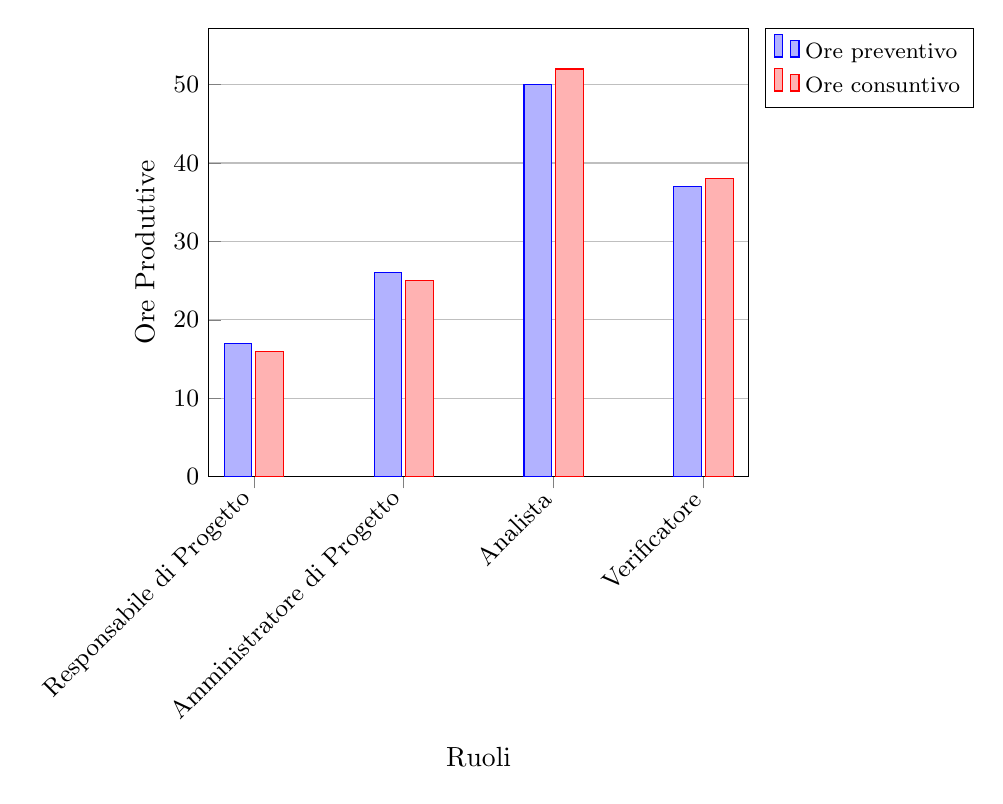
\begin{tikzpicture}
\begin{axis}[
	ybar,
	tick label style={font=\small},
	tickpos=left,
	xlabel = {Ruoli},
	ylabel = {Ore Produttive},
	xticklabels={Responsabile di Progetto, Amministratore di Progetto, Analista, Verificatore}, 
	xtick={1,2,3,4},
	x tick label style = {rotate=45,anchor=east},
	ymin=0,
	ymajorgrids = true,
	legend pos = outer north east,
	legend style = {nodes=right,font=\footnotesize},
]
\addplot +[bar shift=-.2cm] plot coordinates {(1, 17) (2, 26) (3, 50) (4, 37)};

\addplot +[bar shift=.2cm] plot coordinates {(1, 16) (2, 25) (3, 52) (4, 38)};
\legend{\strut Ore preventivo, \strut Ore consuntivo}
\end{axis}
\end{tikzpicture}
\caption{Consuntivo orario, Analisi}
\end{figure}

\subsubsection{Conclusioni}
Dalla tabella~\ref{tab3} si può notare come per svolgere le attività riportate nel diagramma di \gls{Gantt} in figura~\ref{fig1} è stata necessaria un'ora in più di quanto preventivato, con un aumento dei costi di \textbf{15 euro}. Tale passivo non andrà ad influire sul costo totale del progetto in quanto i costi sostenuti in questa macro-fase non vengono poste a carico del Proponente.  

\subsection{Analisi di Dettaglio}
Si riporta di seguito il consuntivo del periodo di \textit{Analisi di Dettaglio}.

\noindent La seguente tabella riporta la differenza di ore impiegate rispetto a quanto preventivato, divise per ruolo. I valori negativi nella tabella indicano un monte ore maggiore di quello preventivato, i valori positivi una diminuzione di ore.

\begin{table}[h]
	\centering
	\begin{tabular}{|l|c|c|}
		\toprule
		\textbf{Ruolo} & \textbf{Ore per ruolo} & \textbf{Costo per ruolo} \\
		
		\midrule
		Responsabile di Progetto & +1 & 20 \\
		Amministratore di Progetto & +1 & 30 \\ 
		Analista & -3 & -75 \\
		Progettista & & \\
		Programmatore & & \\
		Verificatore & +2 & 30 \\
		\midrule
		\textbf{Totale} & +1 & 5 \\
		
		\bottomrule
	\end{tabular}
	\caption{Differenza ore e costo per ruolo, Analisi di Dettaglio}
	\label{tab4}
\end{table} 

\noindent La seguente tabella riporta le differenze tra ore preventivate e quelle impiegate, per membro, durante il periodo di \textit{Analisi di Dettaglio}: 
\begin{table}[h]
	\centering
	\begin{tabular}{|l|c|c|c|c|c|c|c|}
		\toprule
		\textbf{Cognome e Nome} & \multicolumn{6}{c}{\textbf{Ore per ruolo}} & \textbf{Ore Totali} \\
		& \textbf{Re} & \textbf{Am} & \textbf{An} & \textbf{Pt} & \textbf{Pr} & \textbf{Ve} & \\
		
		\midrule
		Agostinetto Matteo & & & -1 & & & +2 & +1 \\
		Burlin Valerio & & & & & & & \\ 
		Carraro Nicola & & +1 & -1 & & & & \\
		Crespan Emanuele & & & & & & & \\
		Ros Fabio & +1 & & -1 & & & & \\
		Suierica Bogdan & & & & & & & \\
		
		\bottomrule
	\end{tabular}
	\caption{Differenza ore a componente per ruolo, Analisi di Dettaglio}
\end{table}

\newpage
\noindent Il seguente grafico riporta la differenza tra le ore preventivate e quelle impiegate, per ruolo, durante il periodo di \textit{Analisi di Dettaglio}:
\begin{figure}[h]
	\centering
	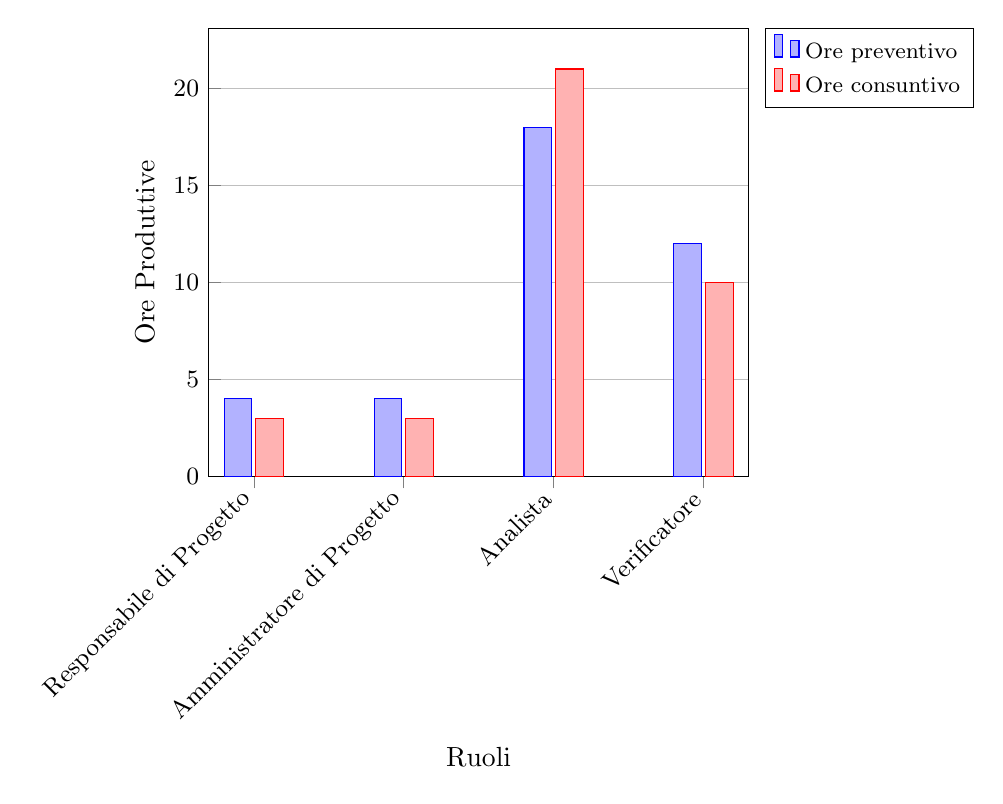
\begin{tikzpicture}
	\begin{axis}[
	ybar,
	tick label style={font=\small},
	tickpos=left,
	xlabel = {Ruoli},
	ylabel = {Ore Produttive},
	xticklabels={Responsabile di Progetto, Amministratore di Progetto, Analista, Verificatore}, 
	xtick={1,2,3,4},
	x tick label style = {rotate=45,anchor=east},
	ymin=0,
	ymajorgrids = true,
	legend pos = outer north east,
	legend style = {nodes=right,font=\footnotesize},
	]
	\addplot +[bar shift=-.2cm] plot coordinates {(1, 4) (2, 4) (3, 18) (4, 12)};
	
	\addplot +[bar shift=.2cm] plot coordinates {(1, 3) (2, 3) (3, 21) (4, 10)};
	\legend{\strut Ore preventivo, \strut Ore consuntivo}
	\end{axis}
	\end{tikzpicture}
	\caption{Consuntivo orario, Analisi di Dettaglio}
\end{figure}

\subsubsection{Conclusioni}
Dalla tabella~\ref{tab4} si può notare come per svolgere le attività riportate nel diagramma di \gls{Gantt} in figura~\ref{fig2} sono state necessarie delle ore in meno per quanto riguarda amministrazione e verifica delle attività, mentre sono state necessarie tre ora in più di quanto preventivato per le attività di \textit{Analista}, al fine di fissare al meglio quanto fatto nel periodo di \textit{Analisi}. Tale pianificazione modificata ha portato ad una diminuzione dei costi di \textbf{5 euro}. Tale attivo non andrà ad influire sul costo totale del progetto in quanto i costi sostenuti in questo periodo non vengono posti a carico del Proponente. 

\subsection{Progettazione Architetturale}
Si riporta di seguito il consuntivo del periodo di \textit{Progettazione Architetturale}.

\noindent La seguente tabella riporta la differenza di ore impiegate rispetto a quanto preventivato, divise per ruolo. I valori negativi nella tabella indicano un monte ore maggiore di quello preventivato, i valori positivi una diminuzione di ore.

\begin{table}[h]
	\centering
	\begin{tabular}{|l|c|c|}
		\toprule
		\textbf{Ruolo} & \textbf{Ore per ruolo} & \textbf{Costo per ruolo} \\
		
		\midrule
		Responsabile di Progetto & +1 & 30 \\
		Amministratore di Progetto & +1 & 20 \\ 
		Analista & -4 & -100 \\
		Progettista & +2 & 44 \\
		Programmatore & & \\
		Verificatore & +1 & 15 \\
		\midrule
		\textbf{Totale} & +1 & 9 \\
		
		\bottomrule
	\end{tabular}
	\caption{Differenza ore e costo per ruolo, Progettazione Architetturale}
	\label{tab5}
\end{table} 

\noindent La seguente tabella riporta le differenze tra ore preventivate e quelle impiegate, per membro, durante il periodo di \textit{Progettazione Architetturale}: 
\begin{table}[h]
	\centering
	\begin{tabular}{|l|c|c|c|c|c|c|c|}
		\toprule
		\textbf{Cognome e Nome} & \multicolumn{6}{c}{\textbf{Ore per ruolo}} & \textbf{Ore Totali} \\
		& \textbf{Re} & \textbf{Am} & \textbf{An} & \textbf{Pt} & \textbf{Pr} & \textbf{Ve} & \\
		
		\midrule
		Agostinetto Matteo & & +1 & & & & & +1 \\
		Burlin Valerio & & & -2 & & & & -2 \\ 
		Carraro Nicola & +1 & & & & & & +1 \\
		Crespan Emanuele & & & & +1 & & & +1 \\
		Ros Fabio & & & & +1 & & +1 & +2 \\
		Suierica Bogdan & & & -2 & & & & -2 \\
		
		\bottomrule
	\end{tabular}
	\caption{Differenza ore a componente per ruolo, Progettazione Architetturale}
\end{table}

\newpage
\noindent Il seguente grafico riporta la differenza tra le ore preventivate e quelle impiegate, per ruolo, durante il periodo di \textit{Progettazione Architetturale}:
\begin{figure}[h]
	\centering
	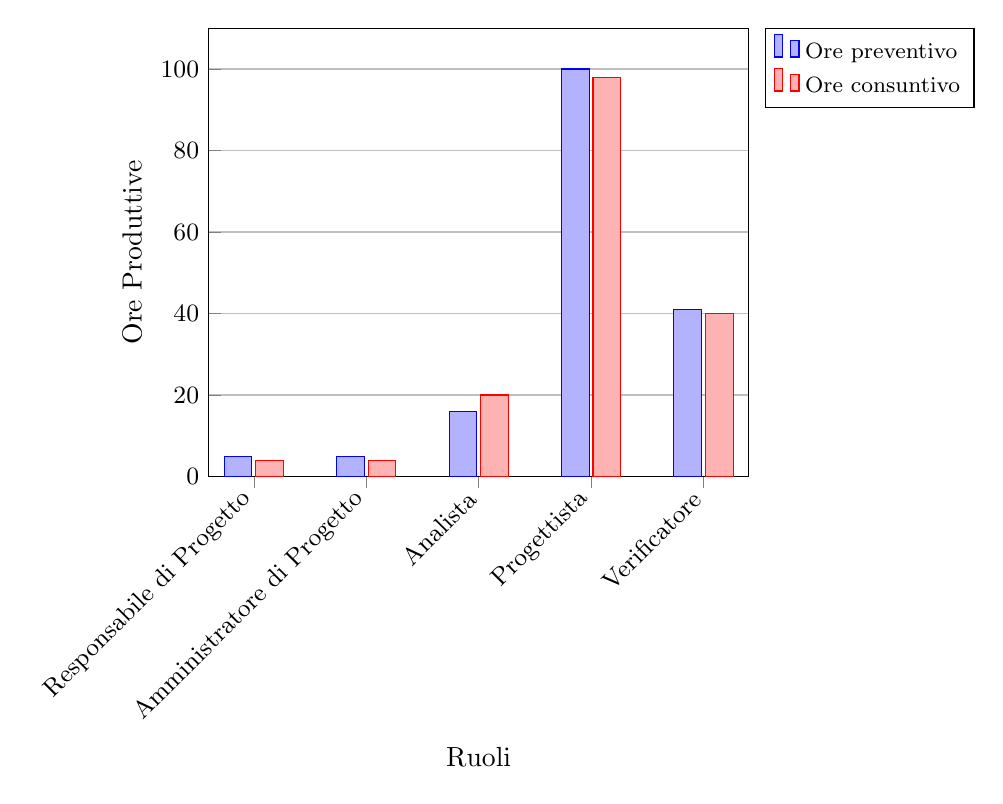
\begin{tikzpicture}
	\begin{axis}[
	ybar,
	tick label style={font=\small},
	tickpos=left,
	xlabel = {Ruoli},
	ylabel = {Ore Produttive},
	xticklabels={Responsabile di Progetto, Amministratore di Progetto, Analista, Progettista, Verificatore}, 
	xtick={1,2,3,4,5},
	x tick label style = {rotate=45,anchor=east},
	ymin=0,
	ymajorgrids = true,
	legend pos = outer north east,
	legend style = {nodes=right,font=\footnotesize},
	]
	\addplot +[bar shift=-.2cm] plot coordinates {(1, 5) (2, 5) (3, 16) (4, 100) (5, 41)};
	
	\addplot +[bar shift=.2cm] plot coordinates {(1, 4) (2, 4) (3, 20) (4, 98) (5, 40)};
	\legend{\strut Ore preventivo, \strut Ore consuntivo}
	\end{axis}
	\end{tikzpicture}
	\caption{Consuntivo orario, Progettazione Architetturale}
\end{figure}

\subsubsection{Conclusioni}
Dalla tabella~\ref{tab5} si può notare come per svolgere le attività riportate nel diagramma di \gls{Gantt} in figura~\ref{fig3} sono state necessarie  quattro ore in più nel ruolo di \textit{Analista} per risolvere e sistemare le carenze del documento \textit{Analisi dei Requisiti} riscontrate durante la Revisione dei Requisiti. Essendo il ruolo di \textit{Analista} uno dei più costosi, si è deciso di pianificare le attività riducendo di qualche ora l'impiego di risorse negli altri ruoli interessati da questo periodo. Tale pianificazione modificata ha portato ad una diminuzione dei costi di \textbf{9 euro}. Tale attivo permette di ottenere un lieve risparmio sul costo totale preventivato del progetto, che potrà essere reimpiegato nelle fasi successive se ritenuto necessario. 
